\documentclass{article}

\usepackage[margin=1in]{geometry}
\usepackage{amsmath}
\usepackage{spverbatim}
\usepackage{graphicx}

\begin{document}
	
\title{ESOF 322 - Homework 4}
\author{Nathan Stouffer and Kevin Browder}

\maketitle
\newpage

\section*{Exercise 1}

\subsection*{Part A}
\subsubsection*{1.}
We downloaded RxJava which is the Reactive Extensions for the Java Virtual Machine.
\subsubsection*{2.}
This library allows you to use Reactive Extension in Java. Reactive extensions is used for asynchronous programming. This library allows you to do asynchronous programming in Java.
\subsubsection*{3.}
This library has about 50,000 lines of code. We calculated this by cloning the repo to a local machine and then using the git ls-files command to determine the number of lines in the documentation (7856) and then determining the number of lines of code in the entire library (57,503). We can then subtract the documentation and find that there are around 50,000 lines of source code.
\subsection*{Part B}
\subsubsection*{1.}
\begin{figure}[h]
	\centering
	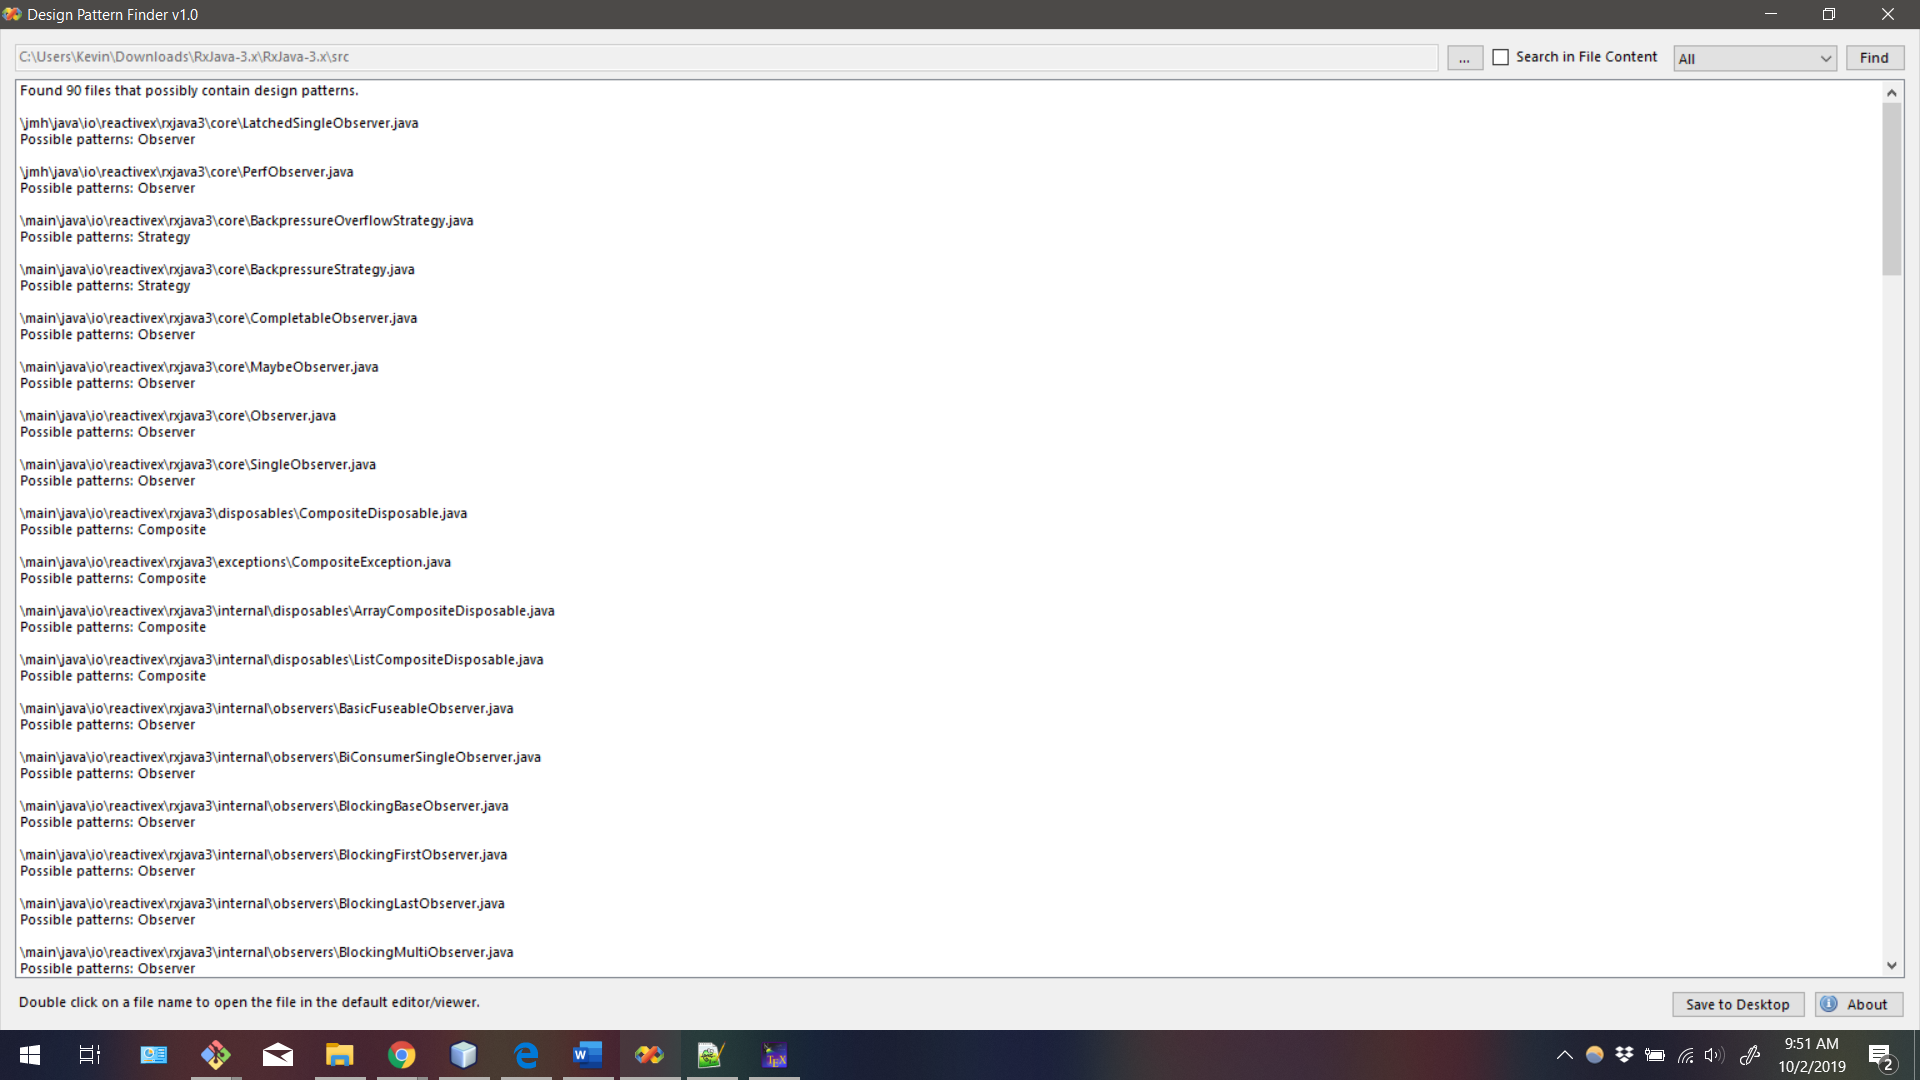
\includegraphics[width=6in]{hw4-patterns.png}
\end{figure}
\subsubsection*{2.}
This program has a set of design pattern definitions in an xml file. It then starts iterating through the file structure and then through the code in each file comparing it to the definitions. If it finds a match it adds that pattern to the output. It then prints all the patterns it found in that file with the file path and then moves to the next file. 
\subsubsection*{3.}
I think I would use a similar design to the DesignPatternTool. All of the design patterns have a pretty distinct signature in code that can be defined. Once these are defined it would be a pretty simple program to use recursion to go through all of the files inside of the directory defined by the user in the program.   


\newpage

\section*{Exercise 2}

\subsection*{Part A}

Question: How did you upload the ESOF 322 files into your Github account? \\\\
Solution: I began by navigating to the esof-322 directory on my computer. I then created a local repository on my computer using the "git init" command. 
I then staged all the subdirectories in esof-322 for a commit. Next, I commited those files with the commit message "initial commit".
Then, on my GitHub account, I created a repository called esof-322.
Finally, I set up the online repository as the remote for my local respository and pushed my initial commit.

\subsection*{Part B}

\end{document}